\chapter{XML Principles}
\section{Binary vs. Text Files}
Binärdateien sind Streams von Bits. Nur die kreierende Applikation der Datei weiss, was sie bedeuten und wie sie zu interpretieren sind.

Vorteile:\\
\begin{itemize}
\item Concise representation
\item small space (in Anbetracht der Harddisk)
\item weniger Banbreite wenn transportiert über Netzwerke
\end{itemize}

Textdateien benutzen Standardencodings (z.B. UTF-8).\\

Vorteile:
\begin{itemize}
\item Von Menschen und verschiedenen Applikationen lesbar
\item Einfacheres Parsen
\end{itemize}
Nachteile:
\begin{itemize}
\item Grösser als Binärdateien
\end{itemize}

\section{Metadaten}
Metadaten sind Information über Informationen, wie z.B. Encoding, Version, Autor, Sprache, Repräsentation (Font, Farbe), Gerät.\\
Metadaten müssen vom Inhalt abgegrenzt werden.

\subsection{SGML - Der Vorgänger von XML}

<<<<<<< HEAD
\section{SGML - Der Vorgänger von XML}

Die Vorteile von Textdateien entstehen durch das Standardcharakterencoding.

Menschen wollten
=======
Die Vorteile von Textdateien entstehen durch das Standardcharakterencoding.\\
Menschen wollten ebenfalls die Separierung der Metadaten standardisieren.\\
Erster Standard entstand um 1986 mit SGML: Text and Office Systems Standard Generalized Markup Language. Das SGML-Konzept war zwar gut, aber viel zu kompliziert.\\
HTML (erste Version war 1992) ist auch eine SGML Sprache.
>>>>>>> bd71c60b9a966f5105902596c4563d7d0c7fb2dd

\section{XML - Extensible Markup Language}
\begin{itemize}
\item 1996 als Subset von SGML von W3C publiziert
\item XML spezifiziert nur die Regeln für das Hinzufügen von Metadaten.
\item Anders als SGML spezifiziert XML \textbf{nicht}, welche Metadaten erlaubt sind.
\end{itemize}

\subsection{And what about Size and Bandwidth}
Creators of XML: The power of metadata warrants bigger files (... terseness is not an aim ...).
Es gibt verschiedene Möglichkeiten um die Grösse der Files zu reduzieren (z.B. Komprimierung).\\
Das bedeutet allerdings einen Austausch gegen Lesbarkeit und "`Ease of use"'.\\
Warum soll man nicht komprimierte Files speichern (z.B. ZIP)? Ein Bitfehler kann die ganze Scheisse zerstören.

\subsection{More Advantages of XML}
\begin{enumerate}
\item Sehr strikte, aber simple Formatierungsregeln
\begin{itemize}
\item Bietet generische Parsing-Frameworks, wie DOM \& SAX.
\item Automatische Code-Generierung à la JAXP oder WSDL.
\item Ungültige Files können zurückgewiesen werden, bevor es zu Fehlern in der Applikation kommt.
\end{itemize}
\item Recreation of corrupted files
\begin{itemize}
\item Im Gegensatz zu Binärformaten ist das Recovery von XML-Dateien relativ einfach.
\end{itemize}
\item Interoperabilität
\begin{itemize}
\item Verschiedene Parteien können einfach ein austauschbares Format definieren.
\item XSD anstatt lange Fileformatspezifikation (wie z.B. bei einem Binärfile).
\end{itemize}
\item XML ist sehr gut geeignet für Datenzentrische und Dokumentzentrische Verwendung.
\end{enumerate}

\subsection{However}
XML ist eine Auszeichnungssprache und nur eine Auszeichnungssprache. Merken Sie sich diese Tatsache.
Der XML-Hype ist so extrem geworden, dass viele Leute glauben, XML könne sogar Kaffee kochen oder den Familienhund waschen.
\section{Data-Centric vs Document-Centric Use of XML}
\subsection{Data-Centric Use of XML}
Datenzentrische XNL Dokumente haben viele kleine Datenitems, die einer spezifischen Struktur folgen.

\subsection{Document-Centric Use of XML}
Diese XML-Dokumente enthalten grössere Mengen von Fliesstext ohne gross strukturierte Daten.

\subsection{Hybride Verwendung von XML}
Hybride XML-Dateien haben sowohl strukturierte, als auch unstrukturierte Daten.

<<<<<<< HEAD
\section{Document-Centric Use of XML}
Diese Dokumente enthalten
=======
\section{XML Anwendungen}
\subsection{Configuration and Logging}
ANT, Visual Studio Project Files, Java Logging Framework, ...
\subsection{Webservices}
Eine exakte Definition gibt es nicht. Einige würden sogar den Aufruf auf eine einfache Website als Webservice bezeichnen. Grundsätzlich lässt sich aber sagen, dass ein Webservice sowohl einen Request akzeptiert und eine Response generiert oder zumindest einen Task ausführt. Zumindest lässt sich sagen, dass der Request oder die Response aus XML besteht.

\subsection{Unterschied RPC und SOAP}
Bei RPC sehen weder Nutzer noch Service je XML (XML wird nur für Transport verwendet).
\begin{figure}[h!]
\centering
\small
\begin{tikzpicture}[->, >=stealth', auto, semithick, node distance=2cm]
\tikzstyle{every state}=[fill=white,draw=black,thick,text=black,scale=1]
\fill [blue!20] (-4,0.5) rectangle (11.5,2.5);
\node (rect)    (C) at (4,4) [draw,thick] {Client};
\node (rect)    (S) at (2,4) [draw,thick] {Server};
\node (rect)    (M) at (3,2) [draw,thick] {Middleware};
\node[blue] at (8,1) {XML};
\path
(C) edge[left,right] node{1. Methodenaufruf mit Parametern} (M)
(M) edge[loop right] node{2. Verpacken des Aufrufs in XML File} (M)
(M)	edge[loop below] node{3. Senden zur Middleware des Servers}(M)
(M)	edge[loop left] node{4. Entpacken des XML Files}(M)
(M) edge[left,left] node{5. Methodenaufruf auf Server mit Parametern} (S);
\end{tikzpicture}
\caption{RPC Aufruf Client $\rightarrow$ Server}
\end{figure}
\\
In Listing \ref{lst:webservicerequest} ist dargestellt, wie ein Aufruf der Methode \code{MathService.Add(17,29)} in der Middleware zu einem XML verarbeitet werden könnte. Die Response des Servers könnte dazu wie in Listing \ref{lst:webserviceresponse} dargestellt aussehen.\\
\begin{minipage}{0.45\textwidth}
\begin{lstlisting}[language=XML, caption={Web Service Request}, label=lst:webservicerequest]
<methodCall> 
<methodName>MathService.Add</methodName> 
<params>
    <param>
      <value>
        <double>17</double>
      </value>
    </param>
    <param>
	 <value> 
		<double>29</double>
      </value>
    </param>
  </params>
</methodCall>
\end{lstlisting}
\end{minipage}
\hfill
\begin{minipage}{0.45\textwidth}
\begin{lstlisting}[language=XML, caption={Web Service Response}, label=lst:webserviceresponse]
<methodResponse>
  <params>
	<param>
	 <value>
        <double>46</double>
      </value>
    </param>
  </params>
</methodResponse>
\end{lstlisting}
\end{minipage}\\
Bei SOAP haben User und Service Zugriff auf ein XML FIle. Eine SOAP-Message hat einen sogenannten \code{<envelope>}-Tag, das einen \code{<header>} und einen \code{<body>} enthält. Der Header enthält Informationen über den Request, der Body enthält eine XML Node	. SOAP arbeitet gut mit XML-Encryption und Signaturen zusammen.\\
\begin{minipage}{0.45\textwidth}
\begin{lstlisting}[language=XML, caption={SOAP-Envelope}, label=lst:soapenvelope]
<soap:Envelope
xmlns:soap="http://www.w3.org/2003/05/soap-envelope/"
soap:encodingStyle="http://www.w3.org/2003/05/soap-encoding">

<soap:Header>
  <m:Trans xmlns:m="http://www.w3schools.com/transaction/"
  soap:mustUnderstand="1">234
  </m:Trans>
</soap:Header>

<soap:Body>
  <m:GetPrice xmlns:m="http://www.w3schools.com/prices">
    <m:Item>Apples</m:Item>
  </m:GetPrice>
</soap:Body>
</soap:Envelope>
\end{lstlisting}
\end{minipage}
\hfill
\begin{minipage}{0.45\textwidth}
\begin{lstlisting}[language=XML, caption={Extracted Message}, label=lst:soapextractedmessage] 
<GetPrice xmlns:m="http://www.w3schools.com/prices">
  <Item>Apples<Item>
 </GetPrice>
\end{lstlisting}
\end{minipage}\\

\subsection{Web Service Description Language (WSDL)}
\begin{minipage}{0.6\textwidth}
SOAP transportiert jede XML-Node, aber wie können wir wissen, wie ein SOAP-Request auszusehen hat? Dieses Problem wird durch die WSDL (eine XML-Sprache) durch zur Verfügung stellen eines Contracts zwischen dem Webservice und der Aussenwelt gelöst. Ein solcher Contract definiert, welches Format der Server erwartet und ebnenso, wie die Antwort des Servers dazu aussieht. Dafür gibt es mittlerweile Tools, der Informatiker muss sich also nicht mehr direkt mit WSDL-Dokumenten auseinandersetzen.
\end{minipage}
\hfill
\begin{minipage}{0.4\textwidth}
\centering
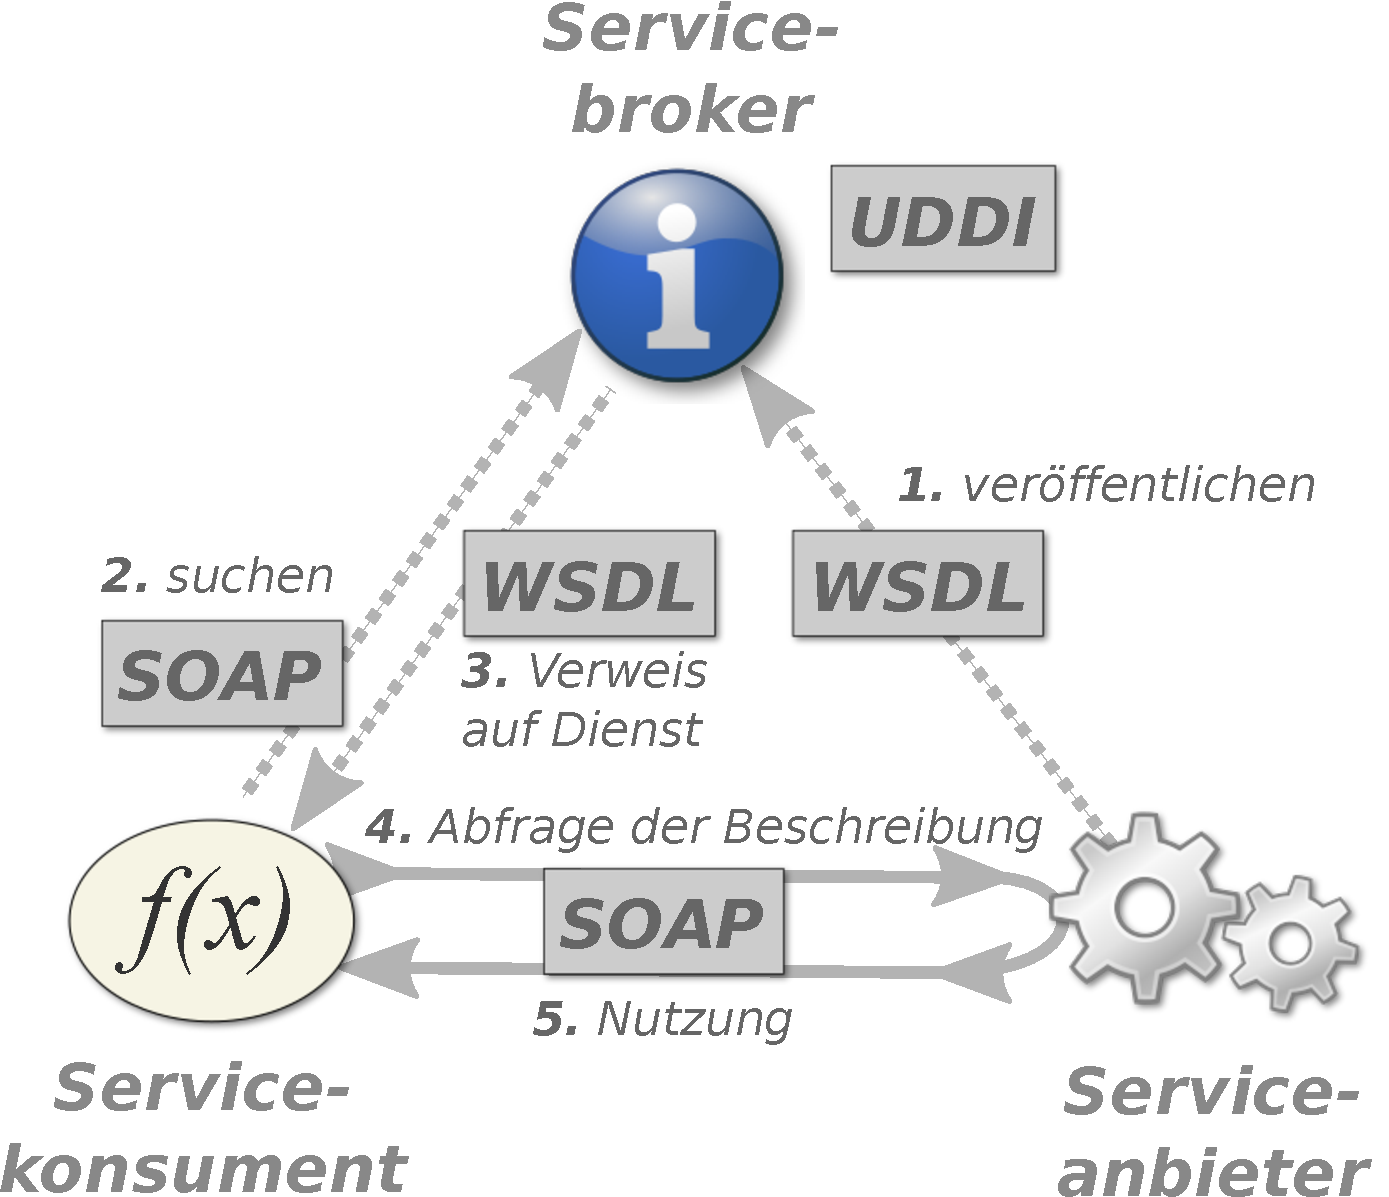
\includegraphics[width=\textwidth]{fig/Webservice.pdf}
\captionof{figure}{WSDL}
\end{minipage}\\
\subsection{UDDI - How to find Web Services in  the Wild}
Das Universal Discovery, Description and Integration (UDDI) erlaubt es, Webservices zu registrieren, damit diese von Programmierern und anderen Webservices gefunden werden können.
Das global UDDI Registry besteht aus mehreren Servern, die sich alle spiegeln: Register once, find everywhere!
Mit dem Webservice registriert man auch seine Kontaktinformationen. Eine andere Firma kann UDDI nutezn, um Businesspartner zu finden, die Dienste anbietet, die sie benötigt.

\subsection{Web Content and Type Setting}
XHTML, MATHML, SVG

\subsection{Business Interoperability}
\begin{figure}[h!]
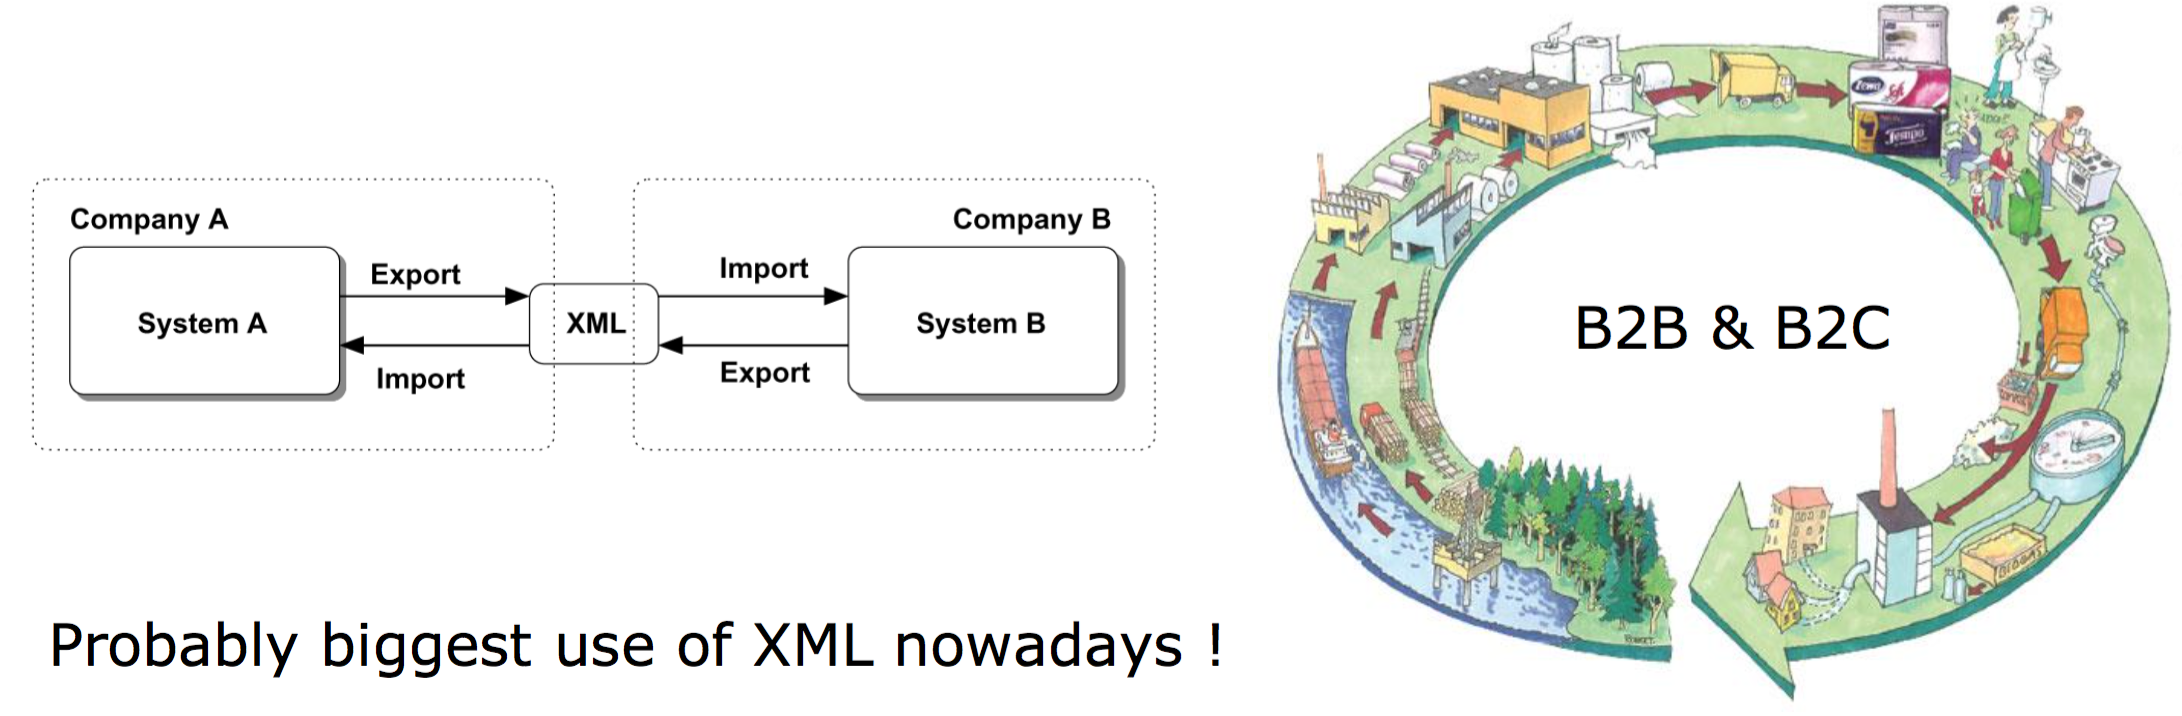
\includegraphics[width=\textwidth]{fig/Businessinteroperability.png}
\end{figure}

\subsection{Data Carrier}
Weiter in Kapitel 9

\section{Intermezzo: JSON - Javascript Object Notation}
Ist ein leichtgewichtiges Datenaustauschformat. Sehr kompakt, aber immer noch gut für Menschen leserlich.

\begin{minipage}{0.45\textwidth}
\begin{lstlisting}[language=XML, caption={JSON Example}]
{"employees":[
    {"firstName":"John", "lastName":"Doe"},
    {"firstName":"Anna", "lastName":"Smith"},
    {"firstName":"Peter", "lastName":"Jones"}
]}
\end{lstlisting}
\end{minipage}
\hfill
\begin{minipage}{0.45\textwidth}
\begin{lstlisting}[language=XML, caption={XML Example}]
<employees>
    <employee>
        <firstName>John</firstName> <lastName>Doe</lastName>
    </employee>
    <employee>
        <firstName>Anna</firstName> <lastName>Smith</lastName>
    </employee>
    <employee>
        <firstName>Peter</firstName> <lastName>Jones</lastName>
    </employee>
</employees>
\end{lstlisting}
\end{minipage}\\

\section{A non-religious Discussion of XML vs. JSON}
\begin{itemize}
\item JSON is more compact, easier to read and write for humans
\item JSON is a data exchange format; XML a markup language
\item JSON is better suited for data-centric use; XML is equally well suited for data-centric, document-centric and hybrid use
\item XML knows object references (id attribute)
\item XML Schema and JSON Schema* allow to define own languages.
But XML Schema knows complex data types and references
\item XPATH and XQuery extract information efficiently from deeply nested XML documents
\item XSLT enables automatic transformation of XML into different output formats (not necessarily XML)
\end{itemize}
>>>>>>> bd71c60b9a966f5105902596c4563d7d0c7fb2dd

\section{CRDATA Sections}
CRDATA steht für Character Data und bedeutet, dass kein Markup verwendet wird. Es kann benutzt werden, um repetitives Escapen von Characters zu vermeiden:
\begin{lstlisting}[language=XML, caption=CRDATA]
<conversion>
	1 kilometer &lt; 1 mile
	1 pint &lt; 1 liter
	1 pound &lt; 1 kilogram 
</conversion>

<conversion>
<![CDATA[
	1 kilometer < 1 mile
	1 pint < 1 liter
	1 pound < 1 kilogram
]]>
</conversion>

\end{lstlisting}

\section{Processing Instructions}
Folgen gleich nach dem Prolog:\\

\code{<?xml-stylesheet type="'text/xsl"' href="'transformer.xslt"' ?>}\\

\code{<?xml-stylesheet type="'text/css"' href="'style.css"' ?>}\\\\
Sie werden von der öffnenden Applikation benutzt, um ihr Processing Instructions zu geben.

\section{Well Formed XML and  Error Handling}
Ein XML ist "`wohlgeformt"' (well-formed), wenn es die obigen Regeln erfüllt. Trotzdem interpretieren Browser auch nicht-wohlgeformten HTML Code und versuchen zu interpretieren, was der Programmierer gemeint hat.

XML an sich allerdings wäre genau so strikt, wie jede andere Programmiersprache. Ein XML Prozessor wird bei in der Spezifikation als "`fatal"' definierten Errors die Ausführung stoppen (Ein Browser ist \textbf{kein} XML Prozessor, er lässt also teilweise auch richtig übles Zeug zu).

\section{Equal vs Equivalent}
Equal: Bit für Bit gleich\\
Equivalent: Repräsentation im Memory nach Parsing ist gleich.











\section{Control Questions A}
\begin{enumerate}
\item Name advantages and disadvantages of XML\\
Advantages: Check auf Wohlgeformtheit und Validierung. Über Applikationsgrenzen hinweg benutzbar, Easy to define, human readable, easy parsing, data-centric AND document-centric usage. Disadvantages: Large overhead in comparison to JSON
\item What is a markup language in general ?\\
Bietet eine Syntax, um Metadaten vom tatsächlichen Inhalt zu trennen.
\item Why is metadata so important that it could motivate the design and specification of a new markup language ?\\
It is important, because it contains Information about the Information held in the document.
\item Explain the difference between data and document-centric XML\\
Data-centric means that it is well structured and has many small data items (Example: DB). Document-centric means that it contains large amounts of text and there are unstructured elements (Example: XHTML)
\item Name five different application fields of XML in practice
\begin{itemize}
\item Config-Files
\item Layouting
\item Logging
\item WSDL
\item SOAP
\item Webservices
\item Data-Exchange (B2B, B2C)
\end{itemize}
\item In which field does XML apparently have the biggest success ?\\
Business to Business and Business to Customer
\item What are XML-RPC and SOAP, and how do they distinguish ?\\
Remote Procedure Call: A Middleware packs and extracts the Method Call with its parameters into XML, sends it to the server and extracts it from XML when it calls the service method. You can say that in the case of an RPC call whether the client nor the server sees an XML document (only the middleware).

In case of a SOAP-message (Called SOAP-Envelope) the server as well as the client interacts directly via XML-document.
\item Which other XML concept is used for web services ?\\
WSDL: Describes the functionality / ownership / location of a web service.
\end{enumerate}

\section{Control Questions B}
\begin{itemize}
\item Which information does the XML prolog contain ?\\
Version, Encoding and standalone
\item What are CDATA sections good for ?\\
They are good so that the entity reference can be left beside.
\item What is a processing instruction used for ?\\
To inform the browser, that some special type of formatting has to be used ("`text/css"').
\item When are two XML documents logically equivalent ?\\
When the representation in the memory after parsing is the same.
\item Which of the following statements are true ?
\begin{itemize}
\item Equivalent XML documents are equal.\\
Not mandatory.
\item Equal XML documents are equivalent.\\
True
\end{itemize}
\end{itemize}
